\documentclass[twoside]{article}

\usepackage{aistats2027}
\usepackage{graphicx}%
\usepackage{multirow}%
\usepackage{amsmath,amssymb,amsfonts}%
\usepackage{amsthm}%
\usepackage{mathrsfs}%
\usepackage[title]{appendix}%
\usepackage{xcolor}%
\usepackage{textcomp}%
\usepackage{manyfoot}%
\usepackage{booktabs}%



\usepackage{listings}%
\usepackage[utf8]{inputenc}
\usepackage[T1]{fontenc}


\usepackage{float}
\newfloat{algorithm}{tbp}{loa}
\floatname{algorithm}{Algorithm}


%% as per the requirement new theorem styles can be included as shown below
\theoremstyle{plain}%
\newtheorem{theorem}{Theorem}%  meant for continuous numbers
%%\newtheorem{theorem}{Theorem}[section]% meant for sectionwise numbers
%% optional argument [theorem] produces theorem numbering sequence instead of independent numbers for Proposition
\newtheorem{proposition}[theorem]{Proposition}% 
%%\newtheorem{proposition}{Proposition}% to get separate numbers for theorem and proposition etc.
\newtheorem{corollary}{Corollary}


\theoremstyle{remark}%
\newtheorem{example}{Example}%
\newtheorem{remark}{Remark}%
\newtheorem{assumption}{Assumption}%

\theoremstyle{definition}%
\newtheorem{definition}{Definition}%

% If your paper is accepted, change the options for the package
% aistats2027 as follows:
%
% \usepackage[accepted]{aistats2027}
%
% This option will print headings for the title of your paper and
% headings for the authors names, plus a copyright note at the end of
% the first column of the first page.

% We also include a `preprint' option for non-anonymous preprints.
% Change the options for the package aistats2027 as follows:
%
%\usepackage[preprint]{aistats2027}
%
% This option will print headings for the title of your paper and
% headings for the authors names, but does not print the copyright and
% venue note at the end of the first column of the first page.

% Submissions have to follow US letter format.
% In case your local TeX installation defaults to A4, you will need to
% set papersize explicitly by activating the following three lines:
% \special{papersize = 8.5in, 11in}
% \setlength{\pdfpageheight}{11in}
% \setlength{\pdfpagewidth}{8.5in}

% If you use the natbib package, activate the following three lines:
\usepackage[round]{natbib}
\renewcommand{\refname}{References}
\renewcommand{\bibsection}{\subsubsection*{\refname}}
\usepackage{hyperref}

% If you use BibTeX in apalike style, activate the following line:
%\bibliographystyle{apalike}

\begin{document}

% If your paper is accepted and the title of your paper is very long,
% the style will print as headings an error message. Use the following
% command to supply a shorter title of your paper so that it can be
% used as headings.
%
%\runningtitle{I use this title instead because the last one was very long}

% If your paper is accepted and the number of authors is large, the
% style will print as headings an error message. Use the following
% command to supply a shorter version of the author names so that
% they can be used as headings (for example, use only the surnames)
%
%\runningauthor{Surname 1, Surname 2, Surname 3, ...., Surname n}

\twocolumn[

\aistatstitle{FusedSpaceFed: Client-Conditioned Input Fusion\\for Heterogeneous Federated Learning}

\aistatsauthor{ Author 1 \And Author 2 \And  Author 3 }

\aistatsaddress{ Institution 1 \And  Institution 2 \And Institution 3 } ]


\begin{abstract}
FusedSpaceFed constructs a client-conditioned classifier input by adding the
original image to an image-shaped residual produced by a private multiscale
encoder and a shared decoder. An encoder-only reconstruction warm-up precedes
joint classification training; only decoder and classifier states are
aggregated. The strongest evidence for this design is its reported performance
against global-model baselines under severe label skew: it has the highest
mean on all twelve MedMNIST tasks at Dirichlet $\alpha=0.05$, and exceeds the
best of FedAvg, FedProx and SCAFFOLD by 11.12--30.45 percentage points on four
two-class-per-client settings. These are descriptive comparisons of existing
means, for which run-level variances are unavailable. We give an exact
fixed-state gradient-dispersion identity and a covariance criterion for
reduction, without claiming that the training dynamics enforce it. The method
adds capacity and computation and is not evaluated under matched budgets.
A separate, fully archived reconstructed FEMNIST study gives
$64.74\pm10.63\%$ sample-weighted accuracy across five seeds and does not
establish superiority to published personalized methods. The evidence
supports a useful client-conditioned alternative to the evaluated global
models in strong label heterogeneity, with explicit limits on causal and
cross-protocol comparisons.
\end{abstract}

\section{Introduction}

Federated learning trains models from distributed client data without
centralizing the training examples \citep{mcmahan2017communication,kairouz2021advances}.
When class proportions differ sharply across clients, repeated local
optimization can produce conflicting updates to a shared classifier.
FedAvg, FedProx and SCAFFOLD address this setting through averaging,
regularization or control variates
\citep{li2018federated,karimireddy2020scaffold}. We study a complementary
intervention: modifying the input supplied to the shared classifier.

For client $i$, FusedSpaceFed classifies
$x+D(E_i(x))$, where $E_i$ is a persistent private encoder and $D$ is a
federated decoder. The original input enters through a fixed additive route, while the learned
pathway supplies a client-conditioned additive signal. Only $D$ and the
classifier are synchronized. Local training first adapts the encoder to the
received decoder using reconstruction MSE, then updates the complete pipeline
using the classification loss. The decoder is optimized for the task in the
second phase; its output is image-shaped but need not remain a faithful
reconstruction.

Our empirical focus is \emph{severe label heterogeneity}. The existing
MedMNIST results show the highest reported mean for FusedSpaceFed on 12/12
tasks at $\alpha=0.05$ and on 4/4 two-class-per-client partitions. In the
latter setting, margins over the highest global-baseline mean are 30.45
points on Path, 22.40 on Derma, 14.89 on Retina and 11.12 on Blood.
At $\alpha=0.50$, margins are smaller and three datasets favor a baseline.
This pattern motivates the scope of the contribution: usefulness relative to
the evaluated global classifiers when a single shared predictor struggles
with label skew, rather than universal dominance across tasks.

Medical federation motivates client-specific representations because sites
can also differ in scanners and acquisition protocols
\citep{sheller2018multi,glocker2019machine,dinsdale2021unlearning,guan2024federated}.
Those physical shifts are not simulated by our MedMNIST partitions: the
experiments vary class allocation, not scanner identity or acquisition
parameters. We therefore do not claim evidence of scanner harmonization,
multi-hospital robustness or clinical fairness.

Personalized federated learning already separates private and shared model
components \citep{arivazhagan2019fedper,collins2021fedrep,li2021ditto,li2021fedbn}.
Our contribution is their particular combination with multiscale private
encoding, shared decoding, additive input fusion and two-phase local training.
The main empirical comparisons are with global baselines and do not isolate
fusion from personalization, added capacity or extra optimization.
A separate reconstructed FEMNIST study is reported in
Section~\ref{sec:femnist_reconstructed}, including every seed: its mean is
below the published FedRep reference and its substantial seed variability
limits claims beyond the main global-baseline comparisons.

The contributions are:
\begin{itemize}
  \item a client-conditioned input pathway with persistent private encoders,
  a shared decoder and classifier, and a precisely specified two-phase update;
  \item an exact classifier-gradient dispersion identity with an explicit
  covariance threshold, interpreted as a diagnostic rather than a convergence
  guarantee;
  \item an evidence-focused analysis of the previously reported medical and
  natural-writer results, plus a separately archived five-seed FEMNIST
  reconstruction; reproducible tables and new figures expose both gains and
  exceptions without imputing missing uncertainties.
\end{itemize}

\section{Background and Related Work}\label{sec:background}

FedAvg alternates local training and parameter averaging
\citep{mcmahan2017communication}. FedProx penalizes deviation from the shared
model \citep{li2018federated}; SCAFFOLD corrects local updates with control
variates \citep{karimireddy2020scaffold}. FedDyn, MOON and FedNTD introduce
dynamic regularization, contrastive representation alignment or prediction
distillation \citep{acar2021feddyn,li2021moon,lee2022preservation}.
These approaches motivate our global-model reference comparisons, but they
do not exhaust the personalized FL design space.

FedPer retains private prediction layers, and FedRep couples a shared
representation with local heads
\citep{arivazhagan2019fedper,collins2021fedrep}. Ditto jointly learns global
and regularized personalized models \citep{li2021ditto}. FedBN keeps
normalization components local to address feature-distribution differences
\citep{li2021fedbn}. FusedSpaceFed instead makes the multiscale mapping to an
additive classifier input private. This supplies a different degree of
client adaptation from head-only or normalization-only personalization:
the private component can change spatial and channel features before the
shared classifier sees them. Sharing the decoder and classifier transfers
task information through that pathway. This is a design rationale, not a
demonstration that local multiscale encoding is necessary or superior to
FedRep, Ditto or FedBN.

Generative federated approaches use learned models to synthesize or distribute
representative samples \citep{tu2021fedcvae,qu2022sdafl,zhang2024fissionvae}.
FusedSpaceFed retains the learned pathway at inference and adds its output
directly to the input. It does not transmit generated samples, but training
and prediction still require local data and computation. Keeping data local
does not itself provide differential privacy or protection against information
leakage from shared updates.

\subsection{Classifier-gradient dispersion}

For a scalar task loss $\ell_{\mathrm{task}}$, let
$F_i(\theta)=\mathbb{E}_{(x,y)\sim\mathcal{D}_i}
[\ell_{\mathrm{task}}(\mathcal{C}_{\theta}(x),y)]$.
At a common classifier state $\theta_t$ and client set $\mathcal{S}_t$,
write $g_{i,t}=\nabla_{\theta}F_i(\theta_t)$,
$m_t=|\mathcal{S}_t|$ and
$\bar g_t=m_t^{-1}\sum_{i\in\mathcal{S}_t}g_{i,t}$.
We use the unnormalized mean-square dispersion
\begin{equation}
\label{eq:gradient_dissimilarity}
\Gamma_t=\frac{1}{m_t}\sum_{i\in\mathcal{S}_t}
\|g_{i,t}-\bar g_t\|_2^2.
\end{equation}
The statistic depends on gradient magnitudes as well as directions. A lower
value alone is not a claim about cosine alignment, progress toward an optimum
or a convergence rate. Heterogeneity affects local optimization
\citep{stich2019localsgd,woodworth2020minibatch}, but our analysis below
conditions on one state and does not model a complete optimization trajectory.


\section{Methodology}\label{sec:method}

\subsection{Private encoding and shared decoding}

Client $i$ has $n_i$ local training samples,
$\mathcal{D}_i=\{(x_j^{(i)},y_j^{(i)})\}_{j=1}^{n_i}$, with
$x\in\mathbb{R}^{c_{\mathrm{in}}\times H\times W}$.
The implementation uses UNetSmallAE with base width 16 and two pooling stages;
$H,W$ are divisible by four (32 in the main experiments, 28 in the separate
reconstruction). Its private encoder returns
\[
E_i(x)=(s_i^{(1)}(x),s_i^{(2)}(x),z_i(x)),
\]
where the skip maps have dimensions
$16\times H\times W$ and $32\times(H/2)\times(W/2)$, and the bottleneck has
dimensions $d_z\times(H/4)\times(W/4)$. Thus $d_z$ is a channel count, not
the total scalar latent dimension. The shared decoder upsamples the bottleneck
and processes both private skip maps \citep{ronneberger2015unet}.

Prediction is based on
\[
\widetilde{x}_i=D_\phi(E_i(x)),\qquad
o_i=\mathcal{C}_\theta(x+\widetilde{x}_i).
\]
The final decoder layer is linear. There is no Sigmoid, output clamp, fusion
coefficient or second normalization after addition. Fusion preserves image
shape but not the original value range. The main studies use a ResNet20-v2
classifier \citep{he2016identity}; the separate reconstructed study uses the
MLP in Section~\ref{sec:femnist_reconstructed}. Both return logits, with the
Softmax operation internal to multiclass cross-entropy rather than applied
before the loss. ChestMNIST uses binary cross-entropy with logits.

\subsection{Two consecutive local phases}\label{sec:training_obj}

At round $t$, $\psi_{i,t}$ is the persistent private encoder and
$(\phi_t,\theta_t)$ are the received shared states. The local working copy
$\psi_i$ is initialized from $\psi_{i,t}$.

\paragraph{Encoder warm-up.}
For $E_w$ epochs, the decoder is frozen and only the encoder is updated using
pixel-mean squared error:
\[
\mathcal L_{\mathrm{rec}}^{(i)}
=\mathbb E_x\left[
\frac{\|x-D_{\phi_t}(E_{\psi_i}(x))\|_2^2}{c_{\mathrm{in}}HW}
\right].
\]
The frozen decoder remains in the computational graph so gradients reach the
encoder. The classifier is inactive and unchanged. This phase attempts to
adapt the private representation to the received decoder; it neither trains
the decoder to reconstruct nor guarantees channel alignment of independently
learned skip maps.

\paragraph{Classification.}
For $E$ epochs, the encoder, decoder and classifier are trainable under
\[
\mathcal L_{\mathrm{cls}}^{(i)}
=\mathbb E_{(x,y)}\left[
\ell_{\mathrm{task}}\!\left(
\mathcal C_{\theta_i}(x+D_{\phi_i}(E_{\psi_i}(x))),y\right)\right].
\]
This phase has no reconstruction penalty. Consequently, the decoder learns a
task-dependent additive residual and can depart from faithful reconstruction.
The direct input term avoids relying on the decoder alone for task features,
but the additive residual can still alter or cancel input information.
The warm-up encourages compatibility with the shared decoder. Neither mechanism
guarantees absence of representation collapse, skip-channel interference or
numerical instability. The separate MLP study required the gradient
stabilization documented in Section~\ref{sec:femnist_reconstructed};
the earlier experiments were not rerun with that modification.

\subsection{Aggregation and persistent state}\label{sec:aggregation}

For the active clients $\mathcal S_t$, only decoder and classifier states are
averaged, uniformly:
\begin{align}
\phi_{t+1}&=\frac{1}{m_t}\sum_{i\in\mathcal S_t}\phi_i^{t+1},
\label{eq:agg_dec}\\
\theta_{t+1}&=\frac{1}{m_t}\sum_{i\in\mathcal S_t}\theta_i^{t+1}.
\label{eq:agg_cls}
\end{align}
The earlier global baselines also use uniform client aggregation.
Encoder states are stored privately as $\psi_{i,t+1}$ and are never
transmitted or averaged. Inactive clients retain $\psi_{i,t+1}=\psi_{i,t}$.
Equal aggregation weight is distinct from weighting test accuracy by samples.

\begin{algorithm}[t]
\caption{FusedSpaceFed with persistent private encoders}
\label{alg:fusedspacefed}
\small
\begin{enumerate}
\item Initialize shared $(\phi_0,\theta_0)$ and private $\psi_{i,0}$.
\item For $t=0,\ldots,T-1$, select $\mathcal S_t$ and broadcast
$(\phi_t,\theta_t)$.
\item For each active client $i$:
  \begin{enumerate}
  \item Restore $\psi_i\gets\psi_{i,t}$;
  initialize $\phi_i\gets\phi_t$, $\theta_i\gets\theta_t$.
  \item Freeze decoder; update only $\psi_i$ for $E_w$ epochs on
  $\mathcal L_{\mathrm{rec}}^{(i)}$.
  \item Unfreeze decoder and classifier; update $\psi_i,\phi_i,\theta_i$
  for $E$ epochs on $\mathcal L_{\mathrm{cls}}^{(i)}$.
  \item Store $\psi_{i,t+1}\gets\psi_i$ privately; upload $(\phi_i,\theta_i)$.
  \end{enumerate}
\item Average only uploaded decoder/classifier states using
Equations~\eqref{eq:agg_dec}--\eqref{eq:agg_cls}; retain inactive encoders.
\end{enumerate}
\end{algorithm}

\subsection{Client-conditioned inference}\label{sec:inference}

After round $T$, client $i$ uses
\[
\widehat y_i=\mathcal C_{\theta_T}
\left(x+D_{\phi_T}(E_{\psi_{i,T}}(x))\right).
\]
The shared classifier and decoder are not a complete standalone predictor.
The medical test protocol measures how each participating client's pathway
performs on a common distribution; the writer and reconstructed FEMNIST
protocols instead use the corresponding client's local test.
No performance on unseen clients is established here. Initializing and
adapting a new encoder would be an additional procedure requiring evaluation.

\section{Gradient-Dispersion Analysis}
\label{sec:theory}

We analyze how dual-space fusion changes the dispersion of
classifier-parameter gradients across clients. At communication round~$t$, the
analysis conditions on the current private encoders, shared decoder, and shared
classifier, allowing the original-input and fused-input gradient fields to be
compared at the same model state.

\subsection{Original and Fused Client Objectives}

Fix a communication round~$t$, an active client set $\mathcal{S}_t$, the shared
classifier parameters $\theta_t$, the shared decoder parameters $\phi_t$, and
the current private encoder parameters $\psi_{i,t}$. During this analysis, all
of these quantities are held fixed except for the argument $\theta$ with
respect to which classifier gradients are defined.
For client~$i$, define the reference original-input objective
\begin{equation*}
F_i^{\mathrm{orig}}(\theta)
=
\mathbb{E}_{(x,y)\sim\mathcal{D}_i}
\left[
\ell_{\mathrm{task}}
\left(
\mathcal{C}_{\theta}(x),y
\right)
\right]
\end{equation*}
and the fused-input objective
\begin{equation*}
\begin{aligned}
F_{i,t}^{\mathrm{fused}}(\theta)
&=\mathbb{E}_{(x,y)\sim\mathcal{D}_i}
\left[\ell_{\mathrm{task}}\left(
\mathcal{C}_{\theta}(u_{i,t}(x)),y\right)\right],\\
u_{i,t}(x)&=x+D_{\phi_t}\!\left(E_{\psi_{i,t}}(x)\right).
\end{aligned}
\end{equation*}
Both are scalar loss functions, and their gradients are taken with respect to
the same classifier parameter vector:
\begin{equation*}
g_{i,t}^{\mathrm{orig}}
=
\nabla_{\theta}F_i^{\mathrm{orig}}(\theta)
\big|_{\theta=\theta_t}, \,\,\,\,\,\,\,
g_{i,t}^{\mathrm{fused}}
=
\nabla_{\theta}F_{i,t}^{\mathrm{fused}}(\theta)
\big|_{\theta=\theta_t}.
\end{equation*}
Define the fusion-induced gradient difference
\begin{equation*}
b_{i,t}
=
g_{i,t}^{\mathrm{fused}}
-
g_{i,t}^{\mathrm{orig}}.
\end{equation*}
Let
\begin{equation*}
\begin{aligned}
\bar{g}_t^{s}
&= \frac{1}{m_t}
   \sum_{i\in\mathcal{S}_t} g_{i,t}^{s},
   \quad s\in\{\mathrm{orig},\mathrm{fused}\},\\
\bar{b}_t
&= \frac{1}{m_t}
   \sum_{i\in\mathcal{S}_t} b_{i,t}.
\end{aligned}
\end{equation*}
where $m_t=|\mathcal{S}_t|$.

\subsection{Exact Fixed-Round Decomposition}

The original and fused classifier-gradient dispersions are
\begin{align*}
\Gamma_t^{\mathrm{orig}}
&=
\frac{1}{m_t}
\sum_{i\in\mathcal{S}_t}
\left\|
g_{i,t}^{\mathrm{orig}}
-
\bar{g}_t^{\mathrm{orig}}
\right\|_2^2,\\
\Gamma_t^{\mathrm{fused}}
&=
\frac{1}{m_t}
\sum_{i\in\mathcal{S}_t}
\left\|
g_{i,t}^{\mathrm{fused}}
-
\bar{g}_t^{\mathrm{fused}}
\right\|_2^2.
\end{align*}

\begin{proposition}[Fixed-round gradient-dispersion identity]
\label{prop:fixed_round_decomposition}
At any fixed round~$t$,
\begin{equation}
\label{eq:exact_decomp}
\Gamma_t^{\mathrm{fused}}
=
\Gamma_t^{\mathrm{orig}}
+
B_t
+
\Phi_t.
\end{equation}
where
\begin{align*}
B_t
&=
\frac{1}{m_t}
\sum_{i\in\mathcal{S}_t}
\left\|
b_{i,t}-\bar{b}_t
\right\|_2^2
\geq 0,\\
\Phi_t
&=
\frac{2}{m_t}
\sum_{i\in\mathcal{S}_t}
\left\langle
g_{i,t}^{\mathrm{orig}}-\bar{g}_t^{\mathrm{orig}},
b_{i,t}-\bar{b}_t
\right\rangle .
\end{align*}
\end{proposition}

\begin{proof}
Because
\begin{equation*}
g_{i,t}^{\mathrm{fused}}
-
\bar{g}_t^{\mathrm{fused}}
=
\left(
g_{i,t}^{\mathrm{orig}}
-
\bar{g}_t^{\mathrm{orig}}
\right)
+
\left(
b_{i,t}-\bar{b}_t
\right),
\end{equation*}
expanding the squared Euclidean norm and averaging over
$i\in\mathcal{S}_t$ gives
\begin{align*}
\Gamma_t^{\mathrm{fused}}
&=
\frac{1}{m_t}
\sum_{i\in\mathcal{S}_t}
\left\|
g_{i,t}^{\mathrm{orig}}
-
\bar{g}_t^{\mathrm{orig}}
\right\|_2^2\\
&\quad+
\frac{1}{m_t}
\sum_{i\in\mathcal{S}_t}
\left\|
b_{i,t}-\bar{b}_t
\right\|_2^2\\
&\quad+
\frac{2}{m_t}
\sum_{i\in\mathcal{S}_t}
\left\langle
g_{i,t}^{\mathrm{orig}}-\bar{g}_t^{\mathrm{orig}},
b_{i,t}-\bar{b}_t
\right\rangle\\
&=
\Gamma_t^{\mathrm{orig}}+B_t+\Phi_t.
\end{align*}
\end{proof}

\begin{corollary}[Fixed-round reduction condition]
\label{cor:fixed_round_reduction}
At the fixed state considered above,
\begin{equation*}
\Gamma_t^{\mathrm{fused}}
<
\Gamma_t^{\mathrm{orig}}
\quad\Longleftrightarrow\quad
B_t+\Phi_t<0.
\end{equation*}
\end{corollary}

The term $B_t$ measures the additional cross-client variability introduced by
the fusion-induced gradient differences. The cross-term $\Phi_t$ is negative
when these differences tend to oppose the original client deviations from
their mean. Therefore, fusion is associated with lower dispersion only when
the negative cross-covariance is sufficiently large to compensate for
$B_t$.


The identity is descriptive and applies whenever the gradient vectors are
finite and defined at the common reference state. Its terms are not estimated
by comparing different methods at their independently trained final states.
In particular, the warm-up and classification losses do not explicitly
minimize $B_t+\Phi_t$.

\paragraph{A quantitative covariance threshold.}
Cauchy--Schwarz gives
$|\Phi_t|\leq 2\sqrt{\Gamma_t^{\mathrm{orig}}B_t}$, hence
\begin{equation}
\label{eq:dispersion_bounds}
\begin{split}
(\sqrt{\Gamma_t^{\mathrm{orig}}}-\sqrt{B_t})^2
&\leq \Gamma_t^{\mathrm{fused}}\\
&\leq(\sqrt{\Gamma_t^{\mathrm{orig}}}+\sqrt{B_t})^2.
\end{split}
\end{equation}
When $\Gamma_t^{\mathrm{orig}}>0$ and $B_t>0$, define
$r_t=\sqrt{B_t/\Gamma_t^{\mathrm{orig}}}$ and
$\rho_t=\Phi_t/(2\sqrt{\Gamma_t^{\mathrm{orig}}B_t})\in[-1,1]$.
Then
\[
\frac{\Gamma_t^{\mathrm{fused}}}{\Gamma_t^{\mathrm{orig}}}
=1+r_t^2+2\rho_t r_t,
\]
so reduction requires $\rho_t<-r_t/2$ and therefore $r_t<2$.
Small reconstruction error alone does not imply this negative covariance.
If $B_t=0$, dispersion is unchanged; if $\Gamma_t^{\mathrm{orig}}=0$,
strict reduction is impossible.

For an illustrative sufficient pattern, suppose
$b_{i,t}=-\lambda(g_{i,t}^{\mathrm{orig}}-\bar g_t^{\mathrm{orig}})+v$,
where $v$ is common to clients. Then
$\Gamma_t^{\mathrm{fused}}=(1-\lambda)^2\Gamma_t^{\mathrm{orig}}$,
which is lower for $0<\lambda<2$ when the original dispersion is positive.
This example assumes the compensating structure; it is not a claim that
UNetSmallAE or the two-phase losses learn it. Positively correlated
corrections can instead increase dispersion.

\paragraph{Scope of the shared-parameter analysis.}
Only classifier gradients are characterized. The shared decoder is also
subject to client drift; it is not assumed negligible, aligned or stable.
The identity does not bound joint $(\theta,\phi)$ dynamics, private-encoder
evolution, multi-step local updates or convergence. The empirical
final-state dispersion measurements below are complementary observations,
not a validation of a negative $\Phi_t$ or of a convergence guarantee.

\subsection{Communication Complexity}

Let $P_C$ and $P_D$ denote the numbers of transmitted scalar values in the
classifier and decoder states, respectively, and let $m_t=|\mathcal{S}_t|$.
At round~$t$, the server sends one classifier and one decoder state to every
active client, and every active client returns the corresponding updated
states. The resulting bidirectional communication is
\begin{equation*}
\mathrm{Comm}_t^{\mathrm{FusedSpaceFed}}
=
2m_t(P_C+P_D)
\end{equation*}
transmitted scalar values, or
$
2m_t(P_C+P_D)b
$
bytes, when each scalar occupies $b$ bytes.

The private encoder is neither uploaded nor downloaded. Relative to FedAvg and
FedProx using the same classifier, FusedSpaceFed therefore communicates an
additional $2m_tP_D$ scalar values per round. For the convolutional decoder,
$P_D$ is determined by the channel widths, convolutional kernels, upsampling
layers, and skip-connection processing blocks. SCAFFOLD additionally maintains
client and server control variates, with communication determined by the
specific control-variate implementation.



\section{Experimental Evidence}\label{sec:experiments}

We organize the evidence around the settings where the reported benefit over
global models is largest, retain moderate-skew exceptions, and separate the
new synthetic-client reconstruction from both the medical studies and natural
writer FEMNIST.

\subsection{Protocols and data availability}

The main MedMNIST study \citep{medmnistv2} uses the official training/test
splits, 10 clients, class-wise Dirichlet allocation and full participation.
The manuscript reports concentrations
$\alpha\in\{0.05,0.1,0.2,0.5,1.0\}$; lower values concentrate client labels.
The alternative pathological allocation restricts each client to two classes.
Every training example is assigned once. These are class-allocation
experiments, not partitions by hospital or scanner.

The reported configuration is 50 rounds, three local classification epochs,
batch 128, uniform aggregation, ResNet20-v2, classifier SGD learning rate
0.01, autoencoder Adam learning rate 0.001
\citep{kingma2015adam}, and FedProx coefficient 0.01.
FusedSpaceFed adds one encoder warm-up epoch. Images from the $64\times64$
release are resized to $32\times32$ and converted to tensors in $[0,1]$.
The baseline and FusedSpaceFed classifier start from the same initialization
and use the same partition within a reported run; this is not equality of
full-model capacity or local compute.

The earlier manuscript describes five runs and validation selection of
$d_z\in\{8,16,32,64\}$ separately per dataset, then a fixed width for test
evaluation and heterogeneity settings. We retain its selected widths.
Original validation traces, per-seed medical results and comparable baseline
tuning records were not available for this revision. Consequently, the
medical means below are preserved aggregates, without recovered SDs,
confidence intervals or significance tests. The implementation and protocol
are available, but exact numerical regeneration of the original runs is not
certified by having runnable entry points.

\paragraph{What the medical test measures.}
Every private encoder, including one trained on two classes, is evaluated
with the final shared decoder/classifier on the \emph{entire official test}.
The reported FusedSpaceFed metric is the uniform mean of the ten pipeline
metrics, not a local-label test or an ensemble of averaged predictions.
Global baselines use their final shared classifier on that same test.
This measures performance on a common test distribution after heterogeneous
training, not accuracy on each client's own test distribution. The shared
classifier sees all participating clients, and the original-input route
remains available, making prediction of locally unseen classes possible;
the aggregates do not identify which pathway causes that generalization.

\paragraph{ChestMNIST.}
The task retains multi-label targets and binary cross-entropy. Partitioning
uses the first positive finding as a proxy stratum, or a no-finding stratum.
Accuracy is mean sample/label agreement after thresholding each output at
0.5. It can be dominated by negative labels and is not evidence of sensitivity,
AUROC, average precision or diagnostic fairness. Those scores cannot be
recovered from aggregate agreement and are not invented here.

\subsection{Severe label skew: the main positive result}\label{sec:strong_skew}

Table~\ref{tab:performance} shows a higher FusedSpaceFed mean than each
global baseline on all twelve tasks at $\alpha=0.05$. The margin over the
highest global-baseline mean ranges from \textbf{0.12 to 7.32 percentage
points}, with notable gains on Path (7.32), Blood (4.96), OCT (3.75) and
Retina (3.31). The small OrganC margin (0.12) is visible rather than rounded
into a claim of a substantial improvement on every task.

% Generated by scripts/build_paper_artifacts.py; do not edit.
\begin{table*}[t]
\centering
\caption{Previously reported MedMNIST mean accuracies (\%) under strong label skew ($\alpha=0.05$). $\Delta$ is FusedSpaceFed minus the highest mean among FedAvg, FedProx and SCAFFOLD, in percentage points. Bold identifies the highest reported mean, not statistical significance. Per-seed records and variances are unavailable; no uncertainty is inferred. Chest accuracy is element-wise label agreement.}
\label{tab:performance}
\small
\setlength{\tabcolsep}{3pt}
\begin{tabular}{lcccccc}
\toprule
Dataset & FedAvg & FedProx & SCAFFOLD & FusedSpaceFed & $d_z$ & $\Delta$ \\
\midrule
Path & 53.45 & 48.11 & 39.90 & \textbf{60.77} & 16 & +7.32 \\
Chest & 90.28 & 89.93 & 89.44 & \textbf{93.22} & 32 & +2.94 \\
Derma & 67.70 & 65.94 & 63.35 & \textbf{69.60} & 16 & +1.90 \\
OCT & 41.56 & 42.50 & 38.69 & \textbf{46.25} & 8 & +3.75 \\
Pneumonia & 69.12 & 70.24 & 70.01 & \textbf{72.95} & 16 & +2.71 \\
Retina & 48.13 & 49.69 & 48.75 & \textbf{53.00} & 64 & +3.31 \\
Breast & 80.25 & 79.33 & 77.78 & \textbf{81.61} & 32 & +1.36 \\
Blood & 53.87 & 47.38 & 45.68 & \textbf{58.83} & 16 & +4.96 \\
Tissue & 35.65 & 33.28 & 34.74 & \textbf{38.21} & 32 & +2.56 \\
OrganA & 23.65 & 25.12 & 19.72 & \textbf{26.01} & 16 & +0.89 \\
OrganC & 22.81 & 24.64 & 18.96 & \textbf{24.76} & 32 & +0.12 \\
OrganS & 22.55 & 21.96 & 20.12 & \textbf{24.11} & 32 & +1.56 \\
\bottomrule
\end{tabular}
\end{table*}


Under the two-class-per-client partitions, FusedSpaceFed's reported
accuracy is 50.94 versus 20.49 on Path, 48.15 versus 25.75 on Derma,
49.26 versus 34.37 on Retina and 30.60 versus 19.48 on Blood, each compared
with the best global mean. The margins, \textbf{11.12--30.45 points}, are
the strongest empirical motivation for the architecture.
Table~\ref{tab:pathological} and Figure~\ref{fig:pathological_means} retain
all methods and all four tasks. These gains support the value of the
complete client-conditioned pipeline in this setting; they do not isolate
additive fusion from personalization, extra capacity or warm-up.

% Generated by scripts/build_paper_artifacts.py; do not edit.
\begin{table*}[t]
\centering
\caption{Previously reported MedMNIST mean accuracies (\%) under two-class-per-client partitions. $\Delta$ is FusedSpaceFed minus the highest mean among FedAvg, FedProx and SCAFFOLD, in percentage points. Bold identifies the highest reported mean, not statistical significance. Per-seed records and variances are unavailable; no uncertainty is inferred. Chest accuracy is element-wise label agreement.}
\label{tab:pathological}
\small
\setlength{\tabcolsep}{3pt}
\begin{tabular}{lccccc}
\toprule
Dataset & FedAvg & FedProx & SCAFFOLD & FusedSpaceFed & $\Delta$ \\
\midrule
Path & 20.49 & 19.66 & 17.16 & \textbf{50.94} & +30.45 \\
Derma & 25.75 & 24.43 & 22.46 & \textbf{48.15} & +22.40 \\
Retina & 34.37 & 33.02 & 26.61 & \textbf{49.26} & +14.89 \\
Blood & 18.22 & 19.48 & 18.10 & \textbf{30.60} & +11.12 \\
\bottomrule
\end{tabular}
\end{table*}


\begin{figure*}[t]
\centering
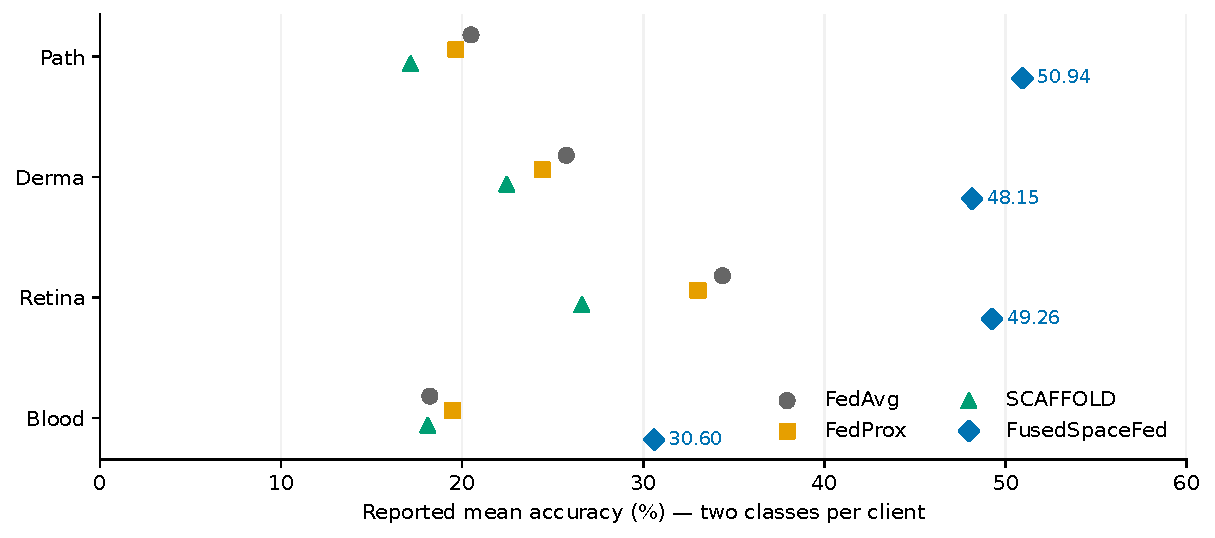
\includegraphics[width=0.95\textwidth]{figures/pathological_accuracy.pdf}
\caption{All reported means on the four two-class-per-client medical
settings. No error bars are drawn because per-run variances are unavailable.
The larger FusedSpaceFed margins are performance comparisons of the full
pipeline against global baselines, not matched-capacity component ablations.}
\label{fig:pathological_means}
\end{figure*}

\subsection{Moderate skew and exceptions}\label{sec:moderate_skew}

At $\alpha=0.50$, FusedSpaceFed has the highest reported mean on 9/12
datasets. The exceptions are \textbf{OCT} (FedProx 70.23 versus 69.88),
\textbf{Blood} (FedAvg 90.43 versus 90.18) and \textbf{OrganS}
(FedAvg 69.56 versus 69.45).
Figure~\ref{fig:mean_gains} shows every dataset at both concentrations,
including these negative margins. The pattern is consistent with greater
usefulness under severe label skew; absent medical variances, the small
differences in either direction are not asserted to be statistically
distinguishable. Chest's agreement metric is interpreted separately from
multiclass accuracy, rather than pooled into a clinical summary score.

% Generated by scripts/build_paper_artifacts.py; do not edit.
\begin{table*}[t]
\centering
\caption{Previously reported MedMNIST mean accuracies (\%) under moderate label skew ($\alpha=0.50$). $\Delta$ is FusedSpaceFed minus the highest mean among FedAvg, FedProx and SCAFFOLD, in percentage points. Bold identifies the highest reported mean, not statistical significance. Per-seed records and variances are unavailable; no uncertainty is inferred. Chest accuracy is element-wise label agreement.}
\label{tab:performance_1}
\small
\setlength{\tabcolsep}{3pt}
\begin{tabular}{lcccccc}
\toprule
Dataset & FedAvg & FedProx & SCAFFOLD & FusedSpaceFed & $d_z$ & $\Delta$ \\
\midrule
Path & 90.49 & 90.70 & 88.38 & \textbf{91.68} & 16 & +0.98 \\
Chest & 94.25 & 93.03 & 93.65 & \textbf{95.25} & 32 & +1.00 \\
Derma & 72.19 & 72.20 & 68.64 & \textbf{72.55} & 16 & +0.35 \\
OCT & 67.72 & \textbf{70.23} & 67.69 & 69.88 & 8 & -0.35 \\
Pneumonia & 82.26 & 81.60 & 82.79 & \textbf{83.42} & 16 & +0.63 \\
Retina & 60.13 & 61.23 & 61.97 & \textbf{62.60} & 64 & +0.63 \\
Breast & 85.35 & 83.34 & 83.43 & \textbf{85.70} & 32 & +0.35 \\
Blood & \textbf{90.43} & 86.51 & 87.00 & 90.18 & 16 & -0.25 \\
Tissue & 61.65 & 59.56 & 60.89 & \textbf{64.33} & 32 & +2.68 \\
OrganA & 81.27 & 81.88 & 80.44 & \textbf{82.23} & 16 & +0.35 \\
OrganC & 79.42 & 77.51 & 79.50 & \textbf{80.16} & 32 & +0.66 \\
OrganS & \textbf{69.56} & 69.17 & 67.50 & 69.45 & 32 & -0.11 \\
\bottomrule
\end{tabular}
\end{table*}


\begin{figure*}[t]
\centering
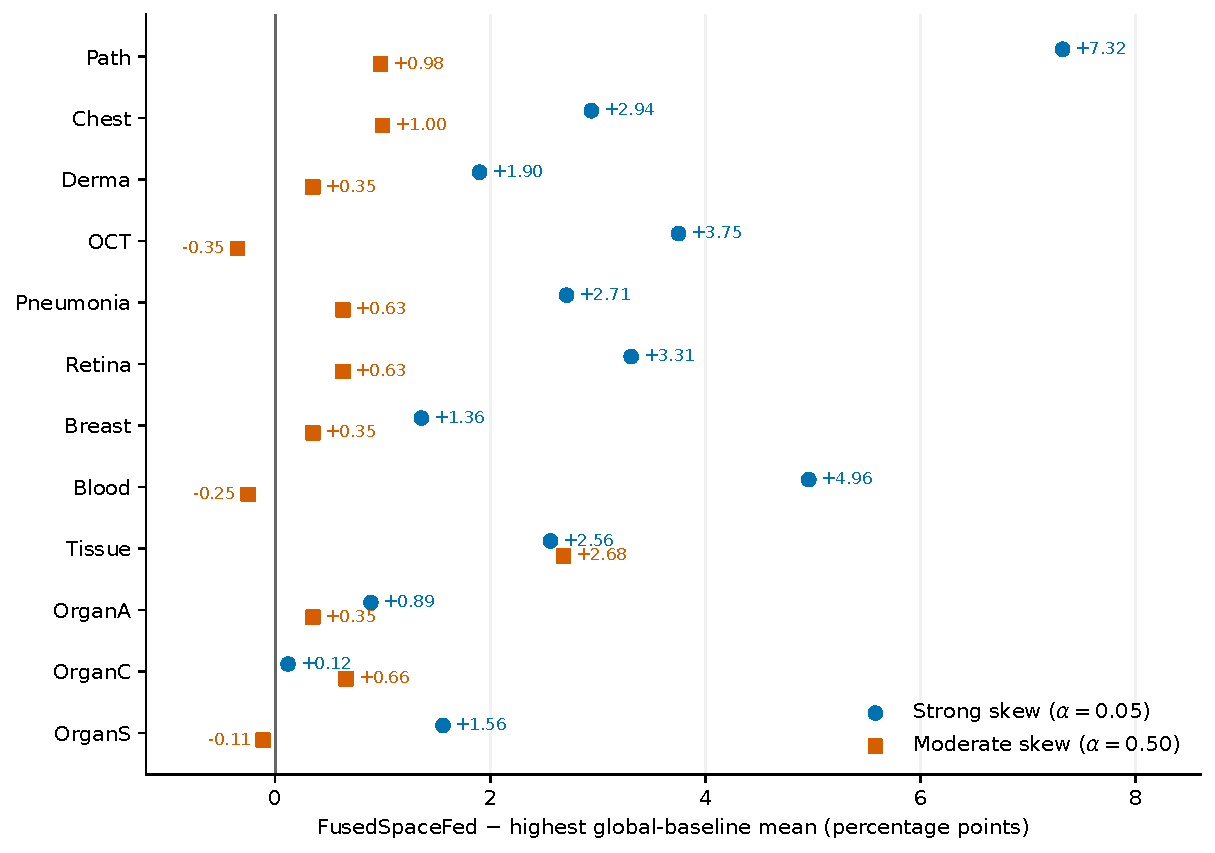
\includegraphics[width=0.95\textwidth]{figures/heterogeneity_gains.pdf}
\caption{FusedSpaceFed minus the highest reported mean of FedAvg, FedProx
and SCAFFOLD per dataset, in percentage points. Both available Dirichlet
settings and all moderate-skew exceptions are displayed. The dots are
differences of archived, rounded means, not paired seed differences;
no missing error bars or significance estimates are inferred.}
\label{fig:mean_gains}
\end{figure*}

\subsection{Gradient dispersion as supporting evidence}

Table~\ref{tab:gradient} retains the reported final-state classifier-gradient
dispersion for four tasks. FusedSpaceFed has the smallest value in each row,
although Retina differs only slightly from FedAvg (9.94 versus 10.05).
One deterministic training minibatch per client estimates the statistic at
each method's \emph{own} final model. Limited batches introduce sampling
sensitivity, and different trained states confound architectural attribution.
These measurements are associated with the favorable accuracy results, but
do not identify the covariance terms at a common state or establish that
fusion caused the reduction. Decoder-gradient dispersion was not measured.
Original PathMNIST stress-sweep renderings are retained in
Appendix~\ref{app:legacy_curves}, with their missing numerical-source limitation.

% Generated by scripts/build_paper_artifacts.py; do not edit.
\begin{table*}[t]
\centering
\caption{Previously reported final-state classifier-gradient dispersion $\Gamma_t$. Methods are measured at their own final states, using a small batch estimate; these are descriptive values, not a same-state test of the decomposition. Per-seed variances and numerical stress-sweep data are unavailable.}
\label{tab:gradient}
\small
\setlength{\tabcolsep}{3pt}
\begin{tabular}{lcccc}
\toprule
Dataset & FedAvg & FedProx & SCAFFOLD & FusedSpaceFed \\
\midrule
Path & 10.68 & 13.89 & 19.91 & \textbf{8.12} \\
Derma & 10.27 & 11.98 & 24.10 & \textbf{8.43} \\
Retina & 10.05 & 10.19 & 42.53 & \textbf{9.94} \\
Blood & 8.65 & 10.14 & 13.60 & \textbf{7.32} \\
\bottomrule
\end{tabular}
\end{table*}


\subsection{Natural-writer FEMNIST: the earlier benchmark}

The earlier FEMNIST study uses natural LEAF writer clients with 62 classes,
not pooled synthetic clients \citep{caldas2018leaf}.
The documented defaults are 50 rounds, three local classification epochs,
one FusedSpaceFed warm-up epoch, batch 256, up to 3400 writers and 340
participants per round, images resized to $32\times32$, and $d_z=64$.
Encoders persist between writer participations. Test predictions use the
corresponding writer's encoder and final shared states; accuracy pools the
local test counts. Gradient dispersion uses one batch from each of 50 seeded
writers.

The preserved aggregates in Table~\ref{tab:femnist_results} favor
FusedSpaceFed: accuracy 86.82 versus the best global value 85.49, macro F1
68.77 versus 66.87, and balanced accuracy 68.38 versus 67.09.
The original $\pm$ values are retained as reported dispersion; without
the original run files, their convention and paired uncertainty cannot be
independently verified. These earlier results are not replaced by the
different reconstruction below.

% Generated by scripts/build_paper_artifacts.py; do not edit.
\begin{table*}[t]
\centering
\caption{Previously reported natural-writer FEMNIST results, kept distinct from the synthetic-client reconstruction. Accuracy, macro F1 and balanced accuracy are percentages; $\Gamma_t$ is gradient dispersion. The original mean $\pm$ dispersion is preserved; per-run records and the uncertainty convention cannot be independently audited.}
\label{tab:femnist_results}
\small
\setlength{\tabcolsep}{3pt}
\begin{tabular}{lcccc}
\toprule
Method & Accuracy & $\Gamma_t$ & Macro F1 & Balanced accuracy \\
\midrule
FedAvg & 85.49 $\pm$ 0.24 & 0.83 $\pm$ 0.01 & 66.87 $\pm$ 0.19 & 67.09 $\pm$ 0.20 \\
FedProx & 84.73 $\pm$ 0.18 & 0.81 $\pm$ 0.02 & 64.16 $\pm$ 0.15 & 65.81 $\pm$ 0.17 \\
SCAFFOLD & 84.51 $\pm$ 0.32 & 0.78 $\pm$ 0.02 & 65.68 $\pm$ 0.26 & 66.46 $\pm$ 0.30 \\
\textbf{FusedSpaceFed} & 86.82 $\pm$ 0.26 & 0.71 $\pm$ 0.02 & 68.77 $\pm$ 0.21 & 68.38 $\pm$ 0.19 \\
\bottomrule
\end{tabular}
\end{table*}


\subsection{Separate reconstructed FEMNIST study}\label{sec:femnist_reconstructed}

This study compares five new FusedSpaceFed runs with \emph{external published
references}, not with baselines trained jointly here. The reference is
Table~1, FEMNIST (150,3), of \citet{collins2021fedrep}.
Our NIST construction uses letters a--j, 150 synthetic clients assigned three
cyclic classes, data seed 20261003 and a frozen local 90/10 split.
Original author splits/seeds are unavailable. To avoid reusing origin images,
insufficient f/i/j pools are allocated by integer proportional reduction with
largest remainders and client-ID tie breaking. This changes class proportions
in 105 clients and yields 25339 examples: 22736 train and 2603 test,
globally disjoint by origin ID. It is \emph{our reconstruction}, not an exact
recovery of the published benchmark.

FusedSpaceFed uses the MLP $784\to512\to256\to64\to10$, ReLU and bias,
raw logits, UNetSmallAE $d_z=64$, 200 rounds, 15 clients/round, batch 10,
one warm-up and five classification epochs. Aggregation is uniform.
Classifier SGD has learning rate 0.01, momentum 0.5 and weight decay
$10^{-4}$ on weights only; AE Adam has learning rate 0.001,
betas $(0.9,0.999)$, $\epsilon=10^{-8}$ and no decay.
Optimizer states reset per participation, with Adam continuous across the
two local phases. Images are $28\times28$, scaled by 255; Float32 is used
without AMP/TF32.

An initial seed-41 attempt became non-finite during round 53, before any test
evaluation. Training-only replay diagnosed exploding classifier gradients
while fused inputs were still finite. We fixed a common L2 gradient clipping
threshold of 1.0 per optimizer, added non-finite checks, and restarted all
five definitive runs from their respective initializations. No test-driven
tuning or seed selection was performed. The failed attempt is preserved
separately and is not counted as a completed run. Clipping controls numerical
failure but does not certify reconstruction quality or uniform convergence.

All final runs completed 200 rounds. Only rounds \textbf{191--200} evaluate
all 150 local tests with current shared states and persistent private encoders,
without adaptation. The primary accuracy pools correct/total counts; the
secondary accuracy averages client accuracies uniformly. Each seed is the
mean of its ten prespecified rounds; the final SD is sample SD across five
run means, not across fifty independent test sets.

% Generated by scripts/build_paper_artifacts.py; do not edit.
\begin{table}[t]
\centering
\caption{Separate reconstructed FEMNIST study: all five run means over rounds 191--200. Both accuracies are percentages; sample SD is across these five means, ddof=1, in percentage points. The first metric is primary. These are not controlled FedRep comparisons.}
\label{tab:femnist_reconstructed}
\small
\setlength{\tabcolsep}{3pt}
\begin{tabular}{lcc}
\toprule
Seed & Sample-weighted & Client-uniform \\
\midrule
41 & 79.5275 & 80.7294 \\
42 & 62.7468 & 62.7314 \\
43 & 63.6650 & 63.2292 \\
44 & 67.8025 & 70.1535 \\
45 & 49.9424 & 49.3587 \\
\midrule
Mean & 64.7368 & 65.2405 \\
Sample SD & 10.6319 & 11.4740 \\
\bottomrule
\end{tabular}
\end{table}


\begin{figure*}[t]
\centering
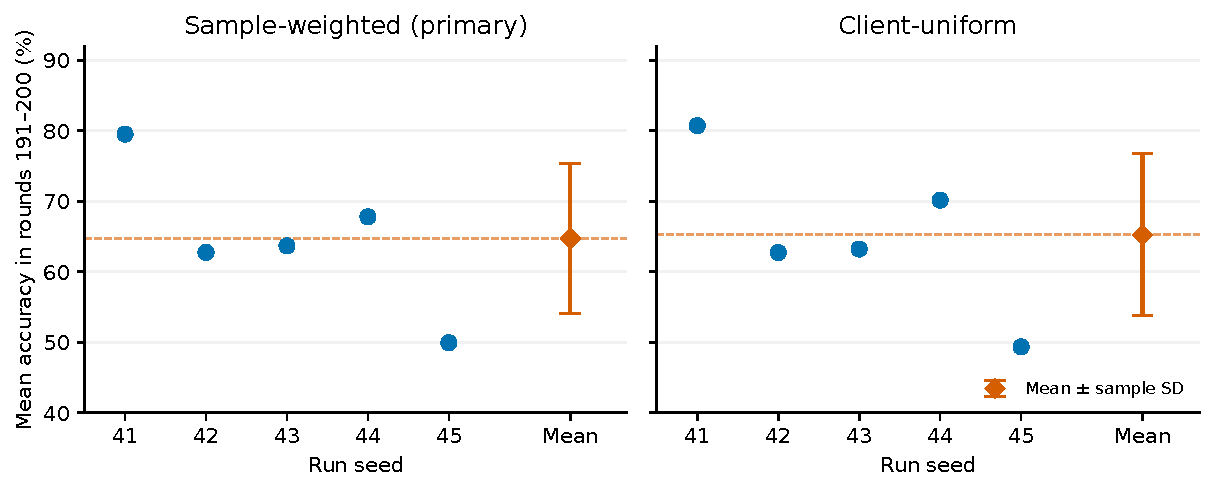
\includegraphics[width=0.95\textwidth]{figures/femnist_reconstructed_seeds.pdf}
\caption{The separate FEMNIST reconstruction, showing every seed for both
metrics. Blue dots are means over rounds 191--200; the orange diamond and
bar are the five-seed mean and sample SD, not a confidence interval.
Published baseline results are not overlaid because this is not a controlled
common experiment.}
\label{fig:femnist_reconstructed_seeds}
\end{figure*}

\paragraph{Outcome and comparability.}
The primary mean is \textbf{$64.74\pm10.63\%$}; the client-uniform mean is
$65.24\pm11.47\%$, with substantial seed dispersion and primary run means
from 49.94 to 79.53. All seeds remain included.
The primary mean is numerically below the published FedRep value
\textbf{78.56\%}; the strongest single seed does not change that outcome.
No superiority over FedRep is established. Original splits, exact execution
commit and seeds are unavailable; historical code and paper descriptions
differ in architecture, Softmax/loss convention, aggregation weights and
test-state handling. Our quota reduction, uniform aggregation, clipping and
additional E/D capacity introduce further differences. Neither the difference
of means nor our SD is a controlled performance estimate or significance test
against FedRep. All published values, with missing uncertainties left missing,
are listed separately in Appendix~\ref{app:reference}.

\paragraph{Measured cost.}
The five processes took 12930.02 s in total, sequentially on one RTX 6000 Ada,
without resumes. Torch allocator peaks were 78.64 MiB allocated and 96 MiB
reserved per run, not including unmeasured driver/context memory; the maximum
RSS was 1544.09 MiB. The MLP has 550346 parameters, the private encoder
71792/client and the decoder 44961, giving 667099 for one pipeline.
The theoretical bidirectional shared-state traffic is 71.44 MB/round,
14.29 GB/run; it is not measured network traffic.
These costs concern this reconstruction only, not the earlier medical runs.
Per-seed costs and identity hashes are in Appendix~\ref{app:costs}.

\subsection{Added capacity and what is not controlled}\label{sec:cost_scope}

Static counts from the implementation put the medical pipeline overhead
$(P_E+P_D)/P_C$ between \textbf{21.0\% and 43.0\%}, depending on $d_z$ and
the task (Table~\ref{tab:model_capacity}). Clients also perform an extra
encoder warm-up and forward/backward through E/D in classification, while
transmitting D as well as C. Equal classifier architecture and classification
epochs therefore do not imply equal total capacity, compute, memory,
communication or validation budget. No matched-budget or component ablation
was performed. The reported advantages concern the complete design over the
evaluated global baselines; they do not prove that additive fusion alone
causes the gains or that it is preferable to other personalized approaches.


\section{Discussion and Conclusion}\label{sec:conclusion}

The strongest result is the consistent advantage of the complete
client-conditioned pipeline over the evaluated global baselines when label
distributions are most concentrated: 12/12 higher reported means at
$\alpha=0.05$ and margins of 11.12--30.45 points in the four two-class
settings. Smaller margins and three exceptions at $\alpha=0.50$ narrow the
claim. The natural-writer aggregates provide a separate positive observation;
the five-seed synthetic reconstruction provides an important counterweight,
with high variability and a mean below the published FedRep reference.

The broader implication is that a shared classifier can be coupled to local
input construction rather than requiring one identical representation for
every client. Our covariance identity makes the requirement for lower
gradient dispersion explicit; it also explains why a learned residual can
increase dispersion when its variability or covariance is unfavorable.
The final-state measurements do not prove that training meets the condition.
The contribution is an empirically useful architectural combination in the
reported strong-skew global-baseline comparisons, not an isolated mechanism,
a convergence guarantee or a claim of superiority across personalized FL.

\subsection{Limitations and practical interpretation}

Direct, controlled comparisons to FedRep, Ditto and FedBN are missing.
Extra capacity, warm-up and validation selection prevent attribution under
equal compute/tuning budgets. Component ablations are unavailable.
The common-test medical evaluation differs from local personalized risk;
real acquisition shifts and unseen clients were not evaluated.
The shared decoder receives classification gradients, not reconstruction
training, and skip alignment or output boundedness is not guaranteed.
The MLP reconstruction's large warm-up losses and frequent clipping show
that finite training need not imply uniformly well-behaved optimization.

Original medical per-run files, stress-sweep numerical data and validation
traces were not recoverable. Mean advantages therefore remain descriptive.
Chest agreement does not establish performance on positive findings.
The fixed-state classifier analysis omits decoder drift and dynamic
convergence. Persistent private encoders add storage and prevent deployment
of the shared components alone. The measured single-GPU costs of the new
study are not measurements of medical clients, distributed networking,
edge energy or baseline cost.

\subsection{Medical, privacy and fairness implications}

No clinical diagnosis, fairness across hospitals or hardware robustness is
validated by class-allocation experiments or aggregate accuracy. Added
resources can constrain low-capacity sites, and aggregate results can conceal
poorly served clients. Client-specific state also raises deployment,
maintenance and access-control requirements. Data locality and omission of
raw-image transfers are not formal privacy guarantees: shared updates can
still expose information. We do not establish resistance to inversion,
membership inference, malicious clients or poisoning. The task residual is
an internal classifier input, not a medically validated image for clinical
interpretation. These limits bound the practical implications of the gains.

\section*{AI Use Statement}

Generative AI tools assisted manuscript editing, analysis scripts and artifact
preparation. Numerical claims are linked to archived sources and automated
checks. Responsibility for the scientific content and final verification
rests with the authors.

\bibliographystyle{apalike}
\clearpage
\bibliography{references}

\clearpage
\appendix
\section{Numerical provenance and reproducible presentation}\label{app:provenance}

The public repository is
\url{https://github.com/CuriosAI/FusedSpaceFed}.
\texttt{scripts/build\_paper\_artifacts.py} regenerates all new tables and
figures without training or evaluating a model. Its \texttt{--check} mode
requires byte-identical outputs. Inputs, outputs, hashes and library versions
are recorded in \path{artifacts/paper_revision/build_manifest.json}.
Legacy values are transcribed from the immutable manuscript at code-history
commit \texttt{fc067b4}; their exact cells and missing uncertainties are in
\path{artifacts/paper_revision/legacy_metrics.csv}.

The five new runs were executed at commit \texttt{cd433ab} with the common
configuration \path{configs/femnist_reconstructed.json}. They are archived
at commit \texttt{fc067b4} in
\path{artifacts/femnist_reconstructed/}, containing losslessly compressed
results, all client counts and timings, a summary and an integrity manifesto.
The configuration and frozen partition are identified by canonical SHA-256
prefixes \texttt{d8684b56bb5d6066} and \texttt{7a4c7614796a595d};
the full hashes are recorded in that manifesto. The seed summary was
independently rebuilt from the client counts before presentation.
The preprocessing and historical protocol discrepancies are documented in
\path{docs/femnist_fedrep_protocol.md}.

Medical means are recoverable as manuscript aggregates; their per-seed
variances are not. The writer table preserves its originally reported
dispersion without relabeling it as a verified SD or confidence interval.
Original JPG curves are a third evidence category: available renderings
without the numerical files needed to regenerate them. These categories are
not conflated with the fully archived new runs.

\section{Static capacity and measured reconstruction costs}\label{app:costs}

% Generated by scripts/build_paper_artifacts.py; do not edit.
\begin{table*}[t]
\centering
\caption{Static parameter accounting from the archived implementation for the medical configurations; no training is performed. C is the shared ResNet classifier, E is one private encoder and D is the shared decoder. Overhead is 100(E+D)/C. These counts quantify added capacity, not measured medical runtime or a matched-budget comparison.}
\label{tab:model_capacity}
\small
\setlength{\tabcolsep}{3pt}
\begin{tabular}{lccccc}
\toprule
Dataset & $d_z$ & C & E & D & Overhead (\%) \\
\midrule
Path & 16 & 272217 & 23600 & 38851 & 22.9 \\
Chest & 32 & 272254 & 34864 & 40865 & 27.8 \\
Derma & 16 & 272087 & 23600 & 38851 & 23.0 \\
OCT & 8 & 271604 & 19264 & 37793 & 21.0 \\
Pneumonia & 16 & 271474 & 23312 & 38817 & 22.9 \\
Retina & 64 & 271669 & 71792 & 44961 & 43.0 \\
Breast & 32 & 271474 & 34864 & 40865 & 27.9 \\
Blood & 16 & 272152 & 23600 & 38851 & 22.9 \\
Tissue & 32 & 271864 & 34864 & 40865 & 27.9 \\
OrganA & 16 & 272059 & 23312 & 38817 & 22.8 \\
OrganC & 32 & 272059 & 34864 & 40865 & 27.8 \\
OrganS & 32 & 272059 & 34864 & 40865 & 27.8 \\
\bottomrule
\end{tabular}
\end{table*}

% Generated by scripts/build_paper_artifacts.py; do not edit.
\begin{table}[t]
\centering
\caption{Measured costs of the five reconstructed runs on one RTX 6000 Ada GPU, run sequentially. Time is the full process wall time; RSS is process RAM. Torch CUDA peaks were 78.64 MiB allocated and 96 MiB reserved in every run, excluding unmeasured driver/context memory.}
\label{tab:reconstructed_costs}
\small
\setlength{\tabcolsep}{3pt}
\begin{tabular}{lcc}
\toprule
Seed & Wall time (min) & RSS (MiB) \\
\midrule
41 & 40.78 & 1544.09 \\
42 & 42.79 & 1540.14 \\
43 & 43.65 & 1541.34 \\
44 & 43.27 & 1531.01 \\
45 & 45.00 & 1529.83 \\
\bottomrule
\end{tabular}
\end{table}


Parameter counts are static properties of the implemented architectures.
The medical classifier has approximately 272000 trainable parameters;
E and D add 57057--116753 parameters in the listed settings.
Transferred classifier state also includes buffers, so state bytes are
counted directly rather than inferred from parameter count alone.
The code reports theoretical upload-plus-download bytes for ten clients in
the medical configurations. This does not measure real network traffic.

The five reconstructed runs used Python 3.12.7, NumPy 2.0.2,
Torch 2.5.1+cu124, CUDA 12.4, cuDNN 9.1.0 and one RTX 6000 Ada GPU.
Each run has one session and no resume. Summed external process time is
12930.02 s; sequencer wall time including inter-run checks is 12930.96 s.
Phase timers are nested in round-compute time, and checkpoint time is nested
in I/O time, so these durations are not additive independent costs.
The five runs recorded 234153 warm-up steps and 1170765 classification steps.
Loss/gradient statistics and per-client participation counts are available in
the archive; their existence does not supply missing measurements for the
earlier medical experiments.

\section{Published FEMNIST references, kept separate}\label{app:reference}

% Generated by scripts/build_paper_artifacts.py; do not edit.
\begin{table}[t]
\centering
\caption{External published references, transcribed from Collins et al., Table 1, FEMNIST (150,3). Accuracy in percent; uncertainties are not reported. No method in this table was rerun here. FusedSpaceFed is deliberately reported in a separate table because datasets/protocols are not controlled jointly.}
\label{tab:fedrep_published}
\small
\setlength{\tabcolsep}{3pt}
\begin{tabular}{lc}
\toprule
Published method & Reported accuracy \\
\midrule
Local Only & 60.86 \\
FedAvg & 51.64 \\
FedAvg+FT & 72.41 \\
FedProx & 18.89 \\
FedProx+FT & 53.54 \\
SCAFFOLD & 17.65 \\
SCAFFOLD+FT & 52.11 \\
Fed-MTL & 54.11 \\
PerFedAvg & 71.51 \\
LG-Fed & 62.08 \\
L2GD & 66.18 \\
APFL & 70.74 \\
Ditto & 68.28 \\
FedPer & 76.91 \\
FedRep & 78.56 \\
\bottomrule
\end{tabular}
\end{table}


This table is reproduced only from the previously verified reference CSV;
the baseline outputs are published values, not our measurements. The authors'
original partition, exact seeds and execution commit are not recovered.
Our construction differs in image allocation and class proportions, and in
documented training/evaluation choices. A comparison of the numerical
levels is contextual, not a controlled or paired statistical comparison.
The published reference does not rescue the missing personalized baselines
in the main common-protocol evaluation.

\section{Original stress-sweep renderings}\label{app:legacy_curves}

The original manuscript describes a PathMNIST stress grid
$\alpha_j=0.05+0.10j$, $j=0,\ldots,11$. Only the following JPG renderings
were available; numerical per-seed curves and their uncertainty calculation
could not be recovered. They are preserved unchanged as historical context,
not used to derive new quantitative margins or convergence claims. The
reproducible mean comparisons in the main text instead use the archived
table values.

\begin{figure*}[t]
\centering
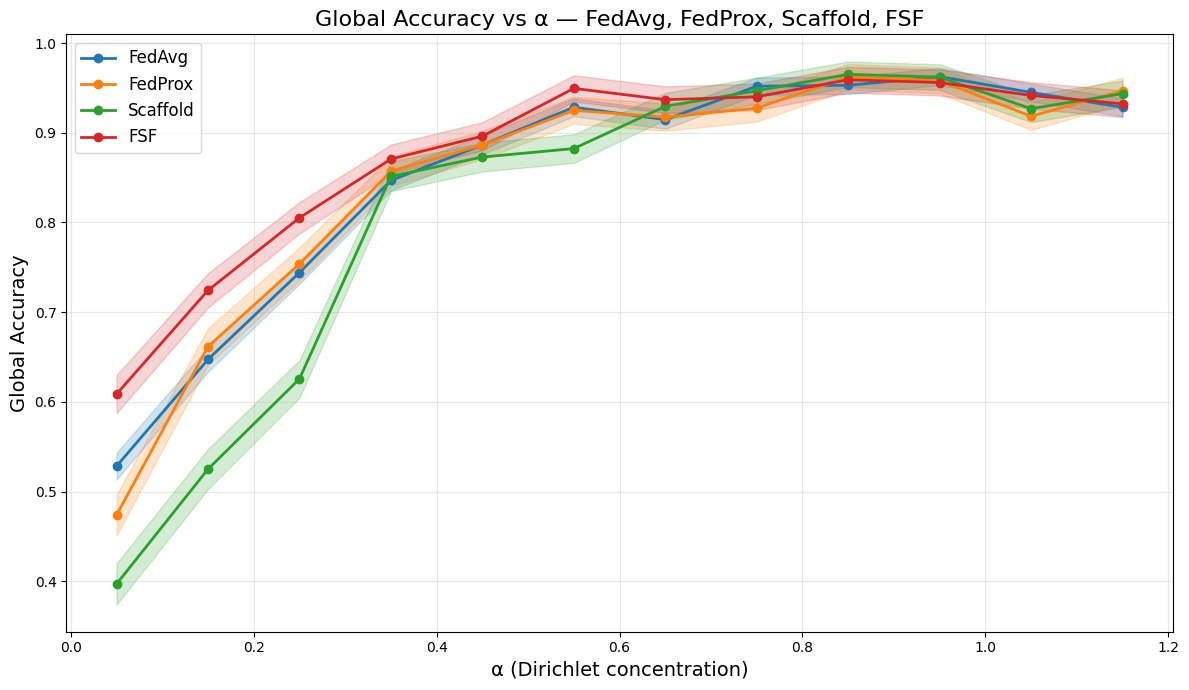
\includegraphics[width=0.95\textwidth]{accuracy_FSF.jpg}
\caption{Original PathMNIST stress-sweep rendering. The legacy legend
\texttt{FSF} means FusedSpaceFed. The original description identifies dots as
five-run means and shading as standard deviation; the underlying numerical
records are unavailable for verification or faithful regeneration.}
\label{fig:dirichlet_breakdown_curve}
\end{figure*}

\begin{figure*}[t]
\centering
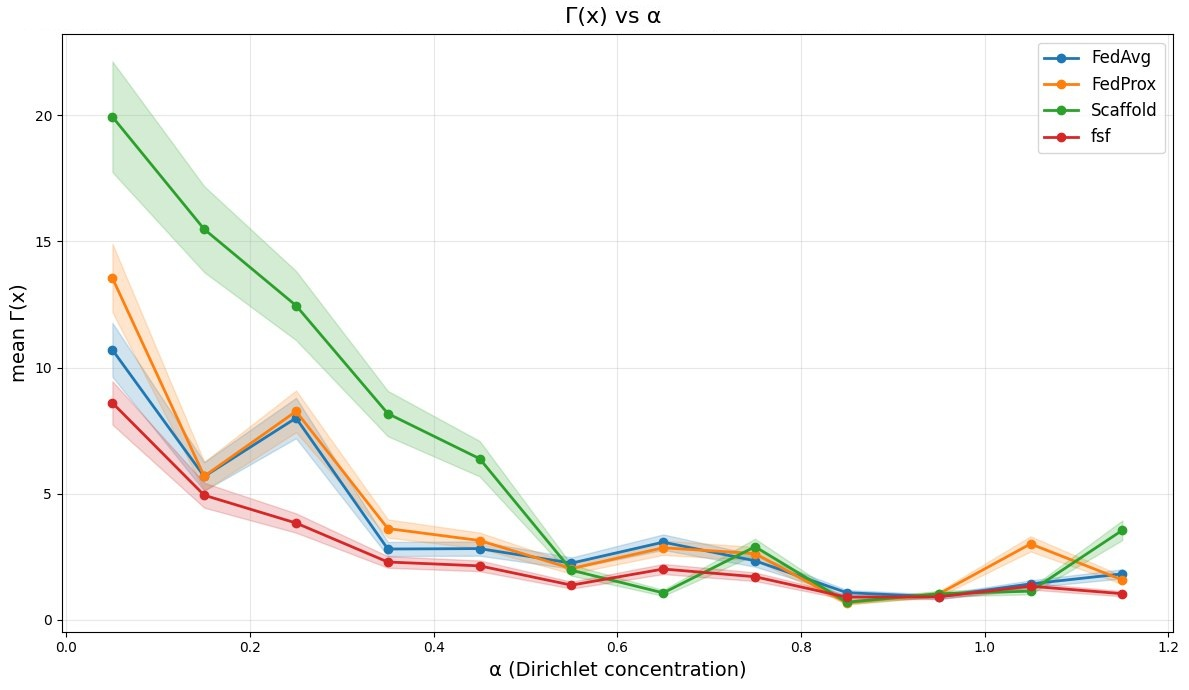
\includegraphics[width=0.95\textwidth]{gamma_FSF.jpg}
\caption{Original dispersion rendering. The legacy axis notation
$\Gamma(x)$ denotes the classifier-gradient statistic $\Gamma_t$, not a
function of an individual image. Mean/standard-deviation shading is retained
as originally described; numerical source records are unavailable. These
method-specific final-state curves do not test the same-state covariance
condition.}
\label{fig:dissimilarity_breakdown_curve}
\end{figure*}

\clearpage
\section*{Checklist}

\begin{enumerate}
\item For all models and algorithms presented, check if you include:
  \begin{enumerate}
  \item A clear description of the mathematical setting, assumptions,
  algorithm, and/or model. [Yes; Sections~\ref{sec:method}--\ref{sec:theory}.]
  \item An analysis of the properties and complexity (time, space, sample
  size) of any algorithm. [Yes; fixed-state properties, communication
  accounting and Appendix~\ref{app:costs}, without convergence or edge-energy claims.]
  \item (Optional) Anonymized source code, with specification of all
  dependencies, including external libraries. [No; code is provided, while
  anonymization is not part of this revision.]
  \end{enumerate}
\item For any theoretical claim, check if you include:
  \begin{enumerate}
  \item Statements of the full set of assumptions of all theoretical
  results. [Yes; finite gradients at a fixed common classifier state.]
  \item Complete proofs of all theoretical results. [Yes; the identity and
  Cauchy--Schwarz derivation in Section~\ref{sec:theory}.]
  \item Clear explanations of any assumptions. [Yes; the compensating
  illustration is explicitly an assumed structure, not a learned guarantee.]
  \end{enumerate}
\item For all figures and tables that present empirical results, check if
you include:
  \begin{enumerate}
  \item The code, data, and instructions needed to reproduce the main
  experimental results (either in the supplemental material or as a URL).
  [No, incomplete; all new presentations and five new run summaries are
  reproducible, but original medical runs and numerical stress curves are
  unavailable. Appendix~\ref{app:provenance} states the scope.]
  \item All the training details (e.g., data splits, hyperparameters, how they
  were chosen). [No, incomplete; reported protocols and the full new
  configuration are supplied, but original validation traces and exact
  historical execution records are missing.]
  \item A clear definition of the specific measure or statistics and error
  bars (e.g., with respect to the random seed after running experiments
  multiple times). [No, incomplete for legacy dispersion; new seed SDs and
  all metric definitions are explicit, with missing uncertainties identified.]
  \item A description of the computing infrastructure used (e.g., type of
  GPUs, internal cluster, or cloud provider). [No for historical runs;
  Appendix~\ref{app:costs} specifies the new study's infrastructure.]
  \end{enumerate}
\item If you are using existing assets (e.g., code, data, models) or
curating/releasing new assets, check if you include:
  \begin{enumerate}
  \item Citations of the creator if your work uses existing assets. [Yes.]
  \item The license information of the assets, if applicable. [No, not a
  complete asset-license audit; provenance is documented separately.]
  \item New assets either in the supplemental material or as a URL, if
  applicable. [Yes; numerical archives and generation scripts.]
  \item Information about consent from data providers/curators.
  [Not Applicable; no new participant data collection.]
  \item Discussion of sensible content if applicable, e.g., personally
  identifiable information or offensive content. [Yes; privacy and medical
  limitations are discussed, and raw data/checkpoints are not published.]
  \end{enumerate}
\item If you used crowdsourcing or conducted research with human subjects,
check if you include:
  \begin{enumerate}
  \item The full text of instructions given to participants and screenshots.
  [Not Applicable.]
  \item Descriptions of potential participant risks, with links to
  Institutional Review Board approvals if applicable. [Not Applicable.]
  \item The estimated hourly wage paid to participants and the total amount
  spent on participant compensation. [Not Applicable.]
  \end{enumerate}
\end{enumerate}

\end{document}
